% !TeX spellcheck = en_GB
% ***************************************************** %
\section{Introduction}\label{sc:intro}
% ***************************************************** %

% problem identification
% solutions

Different SGD-type algorithms proposed by the literature were implemented and tested on different datasets for solving the $\ell_2\text{-regularized}$ Logistic Regression training problem.

For the purpose of this work, those algorithms were grouped into one, see algorithm~\vref{alg:SGD-variants}, follows a list of the variants
\begin{itemize}
\item SGD with fixed or decreasing step-size, and line search, see section~\vref{subsc:sgd};
\item SGD with momentum term and momentum correction or restart, see section~\vref{subsc:sgdm}.
\end{itemize}

%Those algorithms can be divided in basic SGD and SGD with line search due to common computations, follows a list of the implemented algorithms
%\begin{itemize}
%\item Mini-batch Gradient Descent with fixed step-size and momentum term, and decreasing step-size, algorithm~\vref{alg:SGD-F-D-M};
%\item Mini-batch Gradient Descent with Armijo line search and momentum term restart and correction, algorithm~\vref{alg:SGD-SLS-M};
%\end{itemize}

This section describes the Machine Learning (ML) problem and the related optimization problem, then section~\vref{sc:sgds} summarizes the approaches proposed from the retrieved papers. Section~\vref{sc:exp} describes the experiments performed for showing the behaviour of the algorithms on different datasets.

% ---------------------------------------------------- %
\subsection{Classification task}
% ---------------------------------------------------- %

Given a dataset as follows
\[
\mathcal{D}=\set{(x^{(i)},\,y^{(i)})\mid x^{(i)}\in\mathcal{X},\,y^{(i)}\in\mathcal{Y},\,i=1,2,\dots,N}
\]
the general machine learning optimization problem in the context of \emph{supervised learning} is
\[
\min_{w}\func(w)=L(w)+\lambda\Omega(w)\longrightarrow
\begin{cases}
L(w)=\frac{1}{N}\sum_{i=1}^N\ell_i(w) \\[0.5ex]
\Omega_{\ell_2}=\frac{1}{2}\norma{w}_2^2
\end{cases}
\]
where $L(w)$ is the \emph{loss function} which is dived by the total number of samples in the dataset and $\Omega(w)$ is the \emph{regularization term} with its coefficient $\lambda$. There are three regularization possible choices, the $\ell_2$ regularization was chosen for the problem that we want to address. The vector $w$ contains the model weights associated to the dataset features.

The task performed is the \emph{binary classification} (so the allowed values for the response variable are $\mathcal{Y}=\set{-1,1}$), using the Logistic Regression model. The selected loss function is the \emph{log-loss}, for one dataset sample is
\begin{equation}\label{eq:sample_loss}
\ell_i(w)=\log\bigl(1+\exp(-y^{(i)}w^Tx^{(i)})\bigr)
\end{equation}
figure~\vref{subfig:log-loss} shows a plot of the loss function $\ell(uv)=\log\bigl(1+\exp(-uv)\bigr)$ where $u=y^{(i)}$ and $v=w^Tx^{(i)}$.

\subsubsection*{Prediction}

Once the model is trained, we use the sigmoid function, see figure~\vref{subfig:sigmoid}, to classify (as positive or negative class) unseen data as follows
\[
y^{(i)}=
\begin{cases}
1  & \text{if $w^Tx^{(i)}>0.5$} \\
-1 & \text{if $w^Tx^{(i)}\leq0.5$}
\end{cases}
\]


\begin{figure}
\centering
\subfloat[][\emph{Log-loss, equation~\eqref{eq:sample_loss}. $\mathrm{if}\,uv\gg0$ then the example is labelled correctly; $\mathrm{if}\,uv\ll0$ then the label is the wrong one; $\mathrm{if}\,uv\approx0$ then $w$ is the null model.}\label{subfig:log-loss}]%
{%
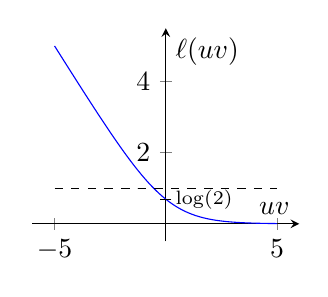
\begin{tikzpicture}
\begin{axis}[xlabel=$uv$,ylabel={$\ell(uv)$},axis lines=middle,enlargelimits,width=0.41\textwidth]
\addplot[samples=200,blue,smooth] {ln(1+exp(-x))};
\addplot[dashed] {1};
\addplot [black, mark=-, nodes near coords=$\log(2)$, font={\scriptsize}, every node near coord/.style={anchor=180}] coordinates {(0,{ln(2)})};
\end{axis}
\end{tikzpicture}%
} \quad
\subfloat[][\emph{Influence of the regularization term on the loss function, equation~\eqref{subeq:obj-fun}, $\lambda=\textcolor{blue}{1},\textcolor{red}{0.5},\textcolor{green}{0.1}$}\label{subfig:loss_regul}]%
{%
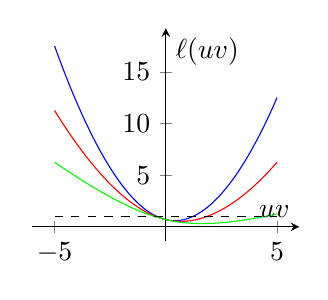
\begin{tikzpicture}
\begin{axis}[xlabel=$uv$,ylabel={$\ell(uv)$},axis lines=middle,enlargelimits,width=0.41\textwidth,legend style={nodes={scale=0.5, transform shape}}]
\addplot[samples=200,blue,smooth] {ln(1+exp(-x))+0.5*x^2};
\addplot[samples=200,red,smooth] {ln(1+exp(-x))+0.5*0.5*x^2};
\addplot[samples=200,green,smooth] {ln(1+exp(-x))+0.5*0.1*x^2};
\addplot[dashed] {1};
%\legend{$\lambda=1$, $\lambda=0.5$, $\lambda=0.1$}
\end{axis}
\end{tikzpicture}
} \quad
\subfloat[][\emph{Sigmoid function. Used for prediction with encoding: $\mathrm{if}\,v>0.5\Rightarrow\hat{u}=1$ and $\mathrm{if}\,v\leq0.5\Rightarrow\hat{u}=-1$.}\label{subfig:sigmoid}]%
{%
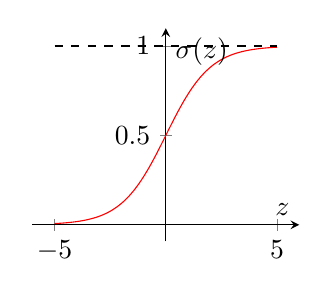
\begin{tikzpicture}
\begin{axis}[xlabel=$z$,ylabel={$\sigma(z)$},axis lines=middle,enlargelimits,width=0.41\textwidth]
\addplot[samples=200,red,smooth] {1/(1+exp(-x))};
\addplot[dashed] {1};
\end{axis}
\end{tikzpicture}%
}
\end{figure}


% ---------------------------------------------------- %
\subsection{Optimization problem}
% ---------------------------------------------------- %

Putting together the loss function and the regularization term, we can obtain the optimization problem that we want to solve using Stochastic Gradient Descent (SGD) algorithm variants
\begin{equation}\label{eq:opt-prob}
%\min_{w\in\R^{(p+1)}}\func(w)=\frac{1}{N}\sum_{i=1}^N\log\bigl(1+\exp(-y^{(i)}w^Tx^{(i)})\bigr)+\lambda\frac{1}{2}\norma{w}^2
\min_{w\in\R^{(p+1)}}\func(w)=\frac{1}{N}\sum_{i=1}^N\log\bigl(1+\exp(-y^{(i)}w^Tx^{(i)})\bigr)+\lambda\frac{1}{2}\norma{w}^2
\end{equation}
where $i=1,\dots,N$ are the dataset samples, $\mathcal{X}\subseteq\R^{(p+1)}$ where $p+1$ means that there are $p$ features and the intercept. %The $1/N$ term isn't always used, we choose to use that term for scaling issues.
We define the matrix associated to the dataset and the model weights as follows
\[
X^T=
\begin{pmatrix}
1 & x_1^{(1)} & x_2^{(1)} & \dots & x_p^{(1)} \\
1 & x_1^{(2)} & x_2^{(2)} & \dots & x_p^{(2)} \\
\vdots & \vdots & \vdots & \ddots & \vdots \\
1 & x_1^{(N)} & x_2^{(N)} & \dots & x_p^{(N)}
\end{pmatrix}\in\R^{N\times(p+1)}\qquad
x^{(i)}=
\begin{pmatrix}
1 \\ x_1^{(i)} \\ x_2^{(i)} \\ \vdots \\ x_p^{(i)}
\end{pmatrix}\quad
w=
\begin{pmatrix}
b \\ w_1 \\ w_2 \\ \vdots \\ w_p
\end{pmatrix}
\]
the constant column is meant for the intercept, also known as \emph{bias}, the $b$ weight in vector $w$. A compact definition for the dataset matrix is $X=(x^{(1)},x^{(2)},\dots,x^{(N)})$.% We can see that every $x^{(i)}$ is a column vector

The objective function $f\colon\R^{(p+1)}\to\R$ is of class $f\in C^2(\R^{(p+1)})$, we compute the first and second order derivatives
\begin{subequations}\label{eq:f-df-ddf}
\begin{align}
%\func(w) &= \frac{1}{N}\sum_{i=1}^N\log\bigl(1+\exp(-y^{(i)}w^Tx^{(i)})\bigr)+\lambda\frac{1}{2}\norma{w}^2 \label{subeq:obj-fun} \\
\func(w) &= \frac{1}{N}\sum_{i=1}^N\log\bigl(1+\exp(-y^{(i)}w^Tx^{(i)})\bigr)+\lambda\frac{1}{2}\norma{w}^2 \label{subeq:obj-fun} \\
%\nabla\func(w) &= \frac{1}{N}Xr+\lambda w \label{subeq:jacobian} \\
\nabla\func(w) &= \frac{1}{N}Xr+\lambda w \label{subeq:jacobian} \\
%\nabla^2\func(w) &= \frac{1}{N}XDX^T+\lambda I_{(p+1)}\label{subeq:hessian}
\nabla^2\func(w) &= \frac{1}{N}XDX^T+\lambda I_{(p+1)}\label{subeq:hessian}
\end{align}
\end{subequations}
where $r\in\R^N$ is a vector of the same length as the total number of samples, whose elements are $r_i=-y^{(i)}\sigma(-y^{(i)}w^Tx^{(i)})$, note that $\sigma(z)$ is the sigmoid function, $D\in\R^{N\times N}$ is a diagonal matrix whose elements are $d_{ii}=\sigma(y^{(i)}w^Tx^{(i)})\sigma(-y^{(i)}w^Tx^{(i)})$ which implies $d_{ii}\in(0,1)$, and $I_{(p+1)}$ is the identity matrix with size $p+1$. Dividing by $N$ means dividing by the total number of samples involved.

The next proposition allows to solve the optimization problem.

\begin{prop}
Problem~\eqref{eq:opt-prob} admits a unique optimal solution.
\end{prop}
\begin{proof}
We need to prove the existence and the uniqueness of the global minimum.

\noindent$(i)$ \emph{Existence} of a optimal solution. The problem is quadratic and the objective function is coercive, in fact $\forall\set{w^k}$ s.t. $\lim_{k\to\infty}\norma{w^k}=\infty$ holds
\[
\lim_{k\to\infty}\func(w^k)\geq\lim_{k\to\infty}\lambda\frac{1}{2}\norma{w^k}^2=\infty\Rightarrow\lim_{k\to\infty}\func(w^k)=\infty
\]
hence by a corollary of the Weirstrass theorem, the problem admits global minimum in $\R^{(p+1)}$.

\noindent$(ii)$ \emph{Unicity} of the optimal solution. We now prove that the hessian matrix~\eqref{subeq:hessian} is positive definite
\[
w^T\nabla^2\func(w)w=w^TXDX^Tw+\lambda w^TIw=\underbrace{y^TDy}_{\geq0}+\lambda\norma{w}^2\geq\lambda\norma{w}^2>0\quad\forall w
\]
the hessian matrix positive definite implies that the objective function is strictly convex and that implies that the global minimum, if exists, is unique. Being in the convex case, the global minimum is a $w^\ast\in\R^{(p+1)}$ s.t. $\nabla\func(w^\ast)=0$ for first-order optimality conditions.\qedhere
\end{proof}

\begin{rmk}
Since the log-loss is convex, the regularization term makes the objective function also \emph{strongly convex}, this should speed up the optimization process.
\end{rmk}

%\begin{rmk}
%further more we can assume that $\nabla\func(w)$ is Lipschitz-continuous with constant $L$
%\end{rmk}

%\begin{itemize}
%\item the hessian matrix is positive defined $\forall w$, this means that the objective function, which is quadratic, is coercive and for the continuity that function admits global minimum, so $\func(w)$ has finite inferior limit
%\item the hessian matrix being positive defined implies also that the objective function is strictly convex (on the other hand the loss function is just convex, due to its hessian matrix being positive semi-defined), this implies that if the global minimum exists, that solution is unique
%\item a global minimum is a point that satisfy $\nabla\func(w^\ast)=0$, which is a sufficient condition implied by the convexity of the problem, see figure~\vref{subfig:log-loss}
%\item the $\ell_2$ regularization implies that the objective function is strongly convex, this speeds up the convergence
%\item further more we can assume that $\nabla\func(w)$ is Lipschitz-continuous with constant $L$
%\end{itemize}
